\documentclass[12pt,a4paper]{article}
\usepackage{graphicx}

\title{IoT-Based Health Monitoring System}

\author{Usman Rasheed Siddiqui}

\date{\today}

\begin{document}

\maketitle

\section{Introduction}

An IoT-based Health Monitoring System is used to monitor a person's
health using sensors and IoT technology. The system collects health
data and sends it to a monitoring application.

\section{Basic Functionality}

The system uses sensors to collect health information such as:

\begin{itemize}
\item Heart rate
\item Body temperature
\item Blood oxygen level
\end{itemize}

The sensors send the collected data to a microcontroller. The
microcontroller sends the data through the Internet to a server.
The user or doctor can then view the health information through a
web or mobile application.

\section{System Components}

The main components of the system are:

\begin{enumerate}
\item Health sensors
\item Microcontroller
\item Internet connection
\item Cloud server
\item Web or mobile application
\end{enumerate}

\section{Block Diagram}

The basic working of the system can be represented as:

\begin{center}
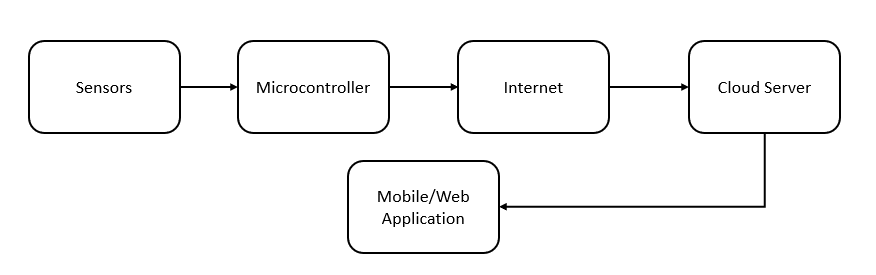
\includegraphics[width=0.9\textwidth]{block_diagram.png}
\end{center}
\section{Conclusion}

The IoT-based Health Monitoring System allows health data to be
collected and monitored remotely. It can help users and doctors
observe important health information easily.

\end{document}
